\chapter{مدل‌های پخشی نویززدای احتمالاتی}
در این فصل به معرفی وبررسی مدل‌های پخشی نویززدای احتمالاتی\LTRfootnote{Denoising diffusion probabilistic models} یا به اختصار مپنا می‌پردازیم. این مدل‌ها نیز از همان قاعده‌ی کلی مدل‌های پخشی که اضافه کردن نویز در یک فرآیند رو به جلو و حذف آن به صورت معکوس است پیروی می‌کنند با این تفاوت که برای این فرآیند از یک زنجیره‌ی احتمالاتی مارکفی استفاده می‌کنند. در این فصل ابتدا به تعریف خود مدل و تابع هزینه‌ی آن می‌پردازیم، سپس با پارامتری سازی مجدد تابع هزینه ، هم ارزی این روش با روش معرفی شده در فصل دوم را نشان می‌دهیم و در نهایت در خصوص فرآیند یادگیری و بهبودهای این مدل مطالبی را مطرح می‌کنیم.

\section{تعریف مدل}
مپناها مدل‌هایی مبتنی بر متغیر پنهان\LTRfootnote{Latent variable models} هستند که از یک زنجیره‌ی مارکفی برای فرآیند پخشی استفاده می‌کنند. رویکرد کلی این مدل‌ها به این صورت است که در یک مسیر رو به جلو هر توزیع پیچیده‌ای از داده‌ها را می‌گیرد و آن را به یک توزیع اولیه که ساده و قابل محاسبه است تبدیل می‌کند و سپس یک مسیر روبه عقب محدود به زمان را یاد می‌گیرد که نمونه هایی از توزیع اولیه را به نمونه‌های توزیع داده تبدیل کند و این همان مدل مولد می‌باشد. تصویر \ref{ddpm1} این فرآیند را نشان می‌دهد. بنابراین این مدل سه مشخصه‌ی اصلی دارد: مسیر رو به جلو، مسیر رو به عقب و تابع مدل مولد که در ادامه هر یک را توضیح می‌دهیم.
\\
\begin{figure}[!h]
	\begin{center}
		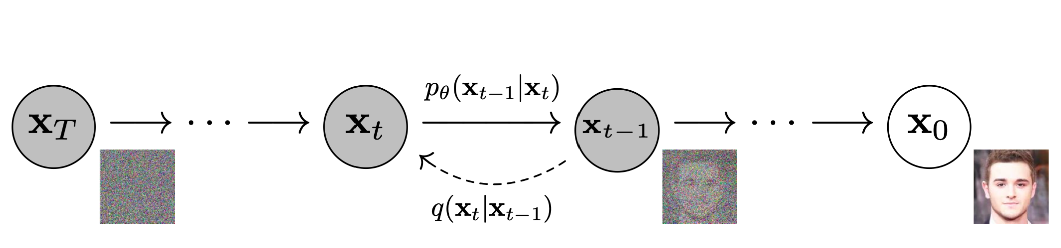
\includegraphics[width=15cm,height=4cm]{ddpm1.png}
		
		\caption{فرآیند پخش در مپناها}
		\medskip
		\label{ddpm1}
		\small
		مدل گرافی جهت‌دار یک مپنا که به صورت یک زنجیره‌ی مارکف روبه جلو و معکوس آن می‌باشد\cite{ho2020denoising}.
		
	\end{center}
\end{figure}


\subsection{مسیر رو به جلو}

اگر توزیع داده را با $q(x^{(0)})$ نشان دهیم، این توزیع به صورت مرحله به مرحله به یک توزیع $\pi(y)$ که از نظر آنالیزی قابل بیان است تبدیل می‌شود و این تبدیل توسط یک هسته‌ي $T_\pi(y|{y}’ ; \beta)$ صورت می‌گیرد که $\beta$ را نرخ پخش\LTRfootnote{Diffusion rate} می‌گوییم وداریم:

\begin{equation}
	\pi(y) = \int dy' \, T_\pi(y|y'; \beta) \pi(y')
\end{equation}

\begin{equation}
	q(x^{(t)} | x^{(t-1)}) = T_\pi(x^{(t)} | x^{(t-1)}}; \beta_t)
	\end{equation}
	
	و بنابراین مسیر رو به جلو\LTRfootnote{Forward trajectory} با شروع از توزیع داده ها و طی $T$ گام پخشی به صورت زیر است:
	
	\begin{equation}
q(x^{(0 \ldots T)}) = q(x^{(0)}) \prod_{t=1}^T q(x^{(t)}|x^{(t-1)})
\end{equation}

در ادامه‌ی این فصل هسته‌ی $ q(x^{(t)} | x^{(t-1)})$ هسته ی گاوسی در نظر گرفته می‌شود اما هسته‌های دیگری چون هسته‌ی دوجمله‌ای\LTRfootnote{Binomial kernel} نیز وجود دارند.
یک ویژگی حائز اهمیت مسیر رو به جلو این است که می‌توان به جای استفاده از فرم زنجیره‌ی مارکفی آن از یک فرم بسته استفاده کرد به این معنا که برای یافتن $x^{(t)}$ در زمان دلخواه $t$ می‌توان از رابطه‌ی زیر کمک گرفت:


\begin{equation}
q(x_t|x_0) = \mathcal{N}(x_t; \sqrt{\overline{\alpha}_t} x_0, (1 - \overline{\alpha}_t)I)
\end{equation}

که $ \overline{\alpha}_t := \prod_{s=1}^t \alpha_s$ و $ \alpha_t := 1 - \beta_t$ تعریف می‌شود.

\subsection{مسیر رو به عقب}

برای یادگیری توزیع مولد نیاز است که بتوانیم برعکس مسیر رو به جلو را یاد بگیریم و این به این معناست که باید بتوانیم از یک توزیع دلخواه قابل محاسبه به توزیع داده برسیم. بنابراین با تعریف توزیع اولیه به صورت $p(x^{(T)}) = \pi(x^{(T)})$ داریم:
\begin{equation}
p(x^{(0 \ldots T)}) = p(x^{(T)}) \prod_{t=1}^T p(x^{(t-1)}|x^{(t)})
\end{equation}
می‌توان نشان داد که اگر فرآیند پخش گاوسی باشد و گام‌های پخش $\beta$ خیلی کوچک باشند آنگاه معکوس فرآیند پخش نیز گاوسی می‌باشد\cite{feller2015retracted}. و بنابراین هر چقدر که طول این زنجیره بیشتر باشد $\beta$ کوچکتر می‌شود و می‌توان از تابع گاوسی برای مسیر معکوس نیز کمک گرفت. در فرآیند یادگیری با توجه به اینکه هسته‌ی گذر\LTRfootnote{Transition kernel} زنجیره ی مارکفی یک تابع گاوسی است، برای ساخت زنجیره تنها نیاز به میانگین و کوواریانس این تابع گاوسی داریم و در ادامه سعی می‌کنیم آنها را تخمین بزنیم.

\subsection{تابع مدل مولد}
تابع احتمال تولید شده توسط مپنا به صورت زیر می‌باشد:

\begin{equation}
p(x^{(0)}) = \int dx^{(1 \ldots T)} p(x^{(0 \ldots T)})
\end{equation}
از آنجاییکه انتگرال در حالت کلی غیرقابل محاسبه\LTRfootnote{Intractable} است، می‌‌توان با ایده گرفتن از نمونه برداری اهمیت\LTRfootnote{Importance sampling} به جای محاسبه‌ی انتگرال از میانگین احتمال نسبی مسیر رو به جلو و مسیر رو به عقب استفاده کرد که به صورت زیر قابل بیان است:



\begin{equation}
p(x^{(0)}) = \int dx^{(1 \ldots T)} q(x^{(1 \ldots T)}|x^{(0)}) \prod_{t=1}^T \frac{p(x^{(t-1)}|x^{(t)})}{q(x^{(t)}|x^{(t-1)})}
\end{equation}

\section{تعریف تابع خطا}
با توجه به مدل تعریف شده در قسمت قبل، آموزش شبکه معادل بیشینه کردن لگاریتم درست‌نمایی\LTRfootnote{Log-likelihood} تابع مدل مولد و یا کمینه کردن منفی این تابع است. بنابراین تابع هزینه را می‌توان به صورت زیر نوشت:


\begin{equation}
L = \int dx^{(0)} q(x^{(0)}) \log p(x^{(0)})
\end{equation}

در اینجا برای آموزش به جای بهینه سازی مستقیم لگاریتم درست‌نمایی از بهینه سازی حد تغییراتی\LTRfootnote{Variational bound} آن کمک می‌گیریم که به صورت زیر قابل تعریف است:

\begin{equation}
\label{vlb}
\mathbb{E}[-\log p_\theta(x^0)] \leq \mathbb{E}_q[-\log \frac{p_\theta(x^{0:T})}{q(x^{1:T}|x^0)}] = \mathbb{E}_q[-\log p(x^T) - \Sigma_{t \geq 1} \log \frac{p_\theta(x^{t-1}|x^{t})}{q(x^t|x^{t-1})}] =: L
\end{equation}

\section{تغییر پارامتر تابع خطا}
از آنجایی که ترکیب مسیر رو به جلو و مسیر معکوس شبیه به یک کدگذار تغییراتی است، می‌توان تابع هزینه را به صورت زیر بازنویسی کرد:

\begin{equation}
\label{total}
\mathcal{L}_{vlb} = \mathcal{L}_0 + \mathcal{L}_1 + \ldots + \mathcal{L}_{T-1} + \mathcal{L}_T
\end{equation}
\begin{equation}
\mathcal{L}_0 = -\log p_\theta(x_0|x_1)
\end{equation}
\begin{equation}
\label{lt1}
\mathcal{L}_{t-1} = \mathcal{D}_{KL}(q(x_{t-1}|x_t, x_0) \| p_\theta(x_{t-1}|x_t))
\end{equation}
\begin{equation}
\mathcal{L}_T = \mathcal{D}_{KL}(q(x_T|x_0) \| p(x_T))
\end{equation}

و از آنجایی که در صورت کوچک بودن $\beta_t$ هر دوی $ p_\theta(x_{t-1}|x_t))$ و $ q(x_{t-1}|x_t, x_0)$ توزیع هایی گاوسی هستند در نتیجه دیورجنس $KL$\LTRfootnote{KL-divergence} آنها را می‌توان به فرم تفاضل میانگین آنها در نظر گرفت و در نتیجه برای معادله ی (\ref{lt1})  داریم:

\begin{equation}
\label{lt2}
\mathcal{L}_{t-1} = \mathbb{E}_q \left[ \frac{1}{2\sigma_t^2} \|\tilde{\mu}_t(x_t, x_0) - \mu_\theta(x_t, t)\|^2 \right] + C
\end{equation} 

که در واقع نشان می‌دهد که در فرآیند آموزش یک مدل پخشی بهینه سازی خطا شامل تخمین میانگین پسین\LTRfootnote{Posterior mean} فرآیند رو به جلو می‌باشد. از طرفی با تغییر پارامتر $ x_t(x_0, \epsilon) = \sqrt{\bar{\alpha_t}}x_0 + \sqrt{(1 - \bar{\alpha_t})}\epsilon$ برای $ \epsilon \sim \mathcal{N}(0, I)$ و قراردهی آن در فرمول معادله‌ی (\ref{lt2}) می‌توان نشان داد که تخمین $\mu_\theta(x_t, t)$ به صورت زیر قابل پارامتری سازی است:

\begin{equation}
\mu_\theta(x_t, t) = \tilde{\mu}_t \left(x_t, \frac{1}{\sqrt{\bar\alpha_t}}\left(x_{t} - \sqrt{1-\bar\alpha_t}\epsilon_\theta(x_t)\right)\right) = \frac{1}{\sqrt{\alpha_t}} (x_t - \frac{\beta_t}{\sqrt{1 - \bar\alpha_t}}\epsilon_\theta(x_t, t)
\end{equation} 

که $\epsilon_\theta$ یک تخمین از نویز موجود در $x_t$ می‌باشد و در نتیجه برای محاسبه ی یک نمونه ی $x_{t-1}$ تنها کافیست که عبارت زیر را محاسبه کنیم:
\begin{equation}
\label{sample}
x_{t-1} = \frac{1}{\sqrt{\alpha_t}} (x_t - \frac{\beta_t}{\sqrt{1 - \bar\alpha_t}}\epsilon_\theta(x_t, t) + \sigma_tz
\end{equation}

که $z$ از توزیع گاوسی با میانگین صفر و کوواریانس همانی می‌ آید.

این تغییر پارامتر دو موضوع مهم را نشان می‌دهد: اول اینکه برای آموزش یک فرآیند رو به عقب می‌توان از تخمین $\tilde{\mu}_t$ با تابع میانگین وابسته به زمان $\mu_\theta$ استفاده کرد و یا مستقیما نویز اضافه شده به داده را با تخمین $\epsilon$ محاسبه کرد. دوم اینکه در حالتی از پارامتری سازی که از تخمین نویز در هر گام زمانی استفاده می‌کنیم در واقع فرآیندی مشابه تطبیق امتیاز نویززدا با دینامیک لانژوین را طی می‌کنیم و در این حالت تابع هدف شبکه را تبدیل به یک مدل تطبیق امتیاز نویززدا می‌کنیم.

\section{فرآیند یادگیری}
با توجه به تغییر پارامتر انجام شده در قسمت قبل و همچنین به کارگیری آن درمعادله‌ی ( \ref{total}) می توان به تابع هزینه ای رسید که کاملا نسبت به $\theta$ مشتق پذیر است و برای آموزش مناسب است اما برای سادگی پیاده سازی و افزایش کیفیت نمونه‌های تولیدی می‌توان تابع هزینه را به شکل زیر نیز بازنویسی کرد:

\begin{equation}
\label{loss}
L_{simple}(\theta) = \mathbb{E}_{t,x_0,\epsilon} \left[ \left \| \epsilon - \epsilon_\theta(\sqrt{\bar\alpha_t}x_0 + \sqrt{1-\bar\alpha_t}\epsilon, t) \right \|^2 \right]
\end{equation} 

که $t$ از یک توزیع یونیفرم بین ۱و $T$ می آید و واریانس $\beta_t$ در این فرآیند یک پارامتر ثابت بدون یادگیری می‌باشد.
در ساختار مپناها از هسته ی اصلی $pixelCNN++$ \cite{salimans2017pixelcnn++} استفاده شده است که در واقع نوعی شبکه‌ی یو با اتصالات گسترده‌ی باقی‌مانده‌ای می‌باشد. شکل\ref{ddpm2} ساختار کلی شبکه‌ی به کار گرفته شده را نشان می‌دهد.

\\
\begin{figure}[!h]
	\begin{center}
		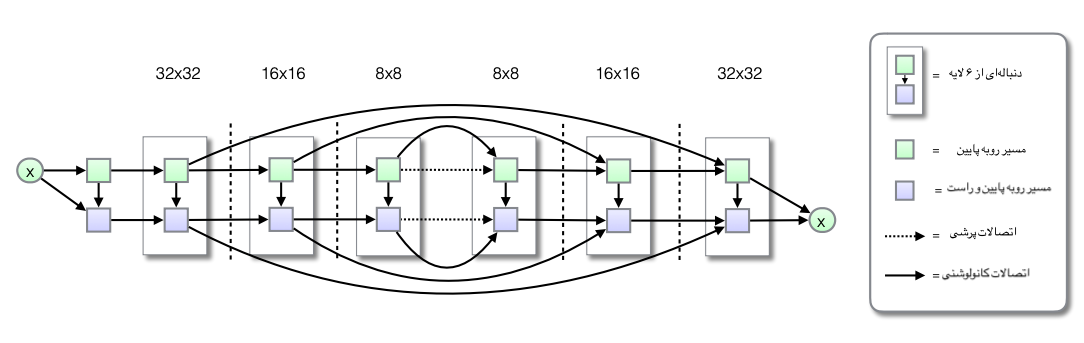
\includegraphics[width=15cm,height=5cm]{ddpm2.png}
		
		\caption{معماری $pixelCNN++$}
		\medskip
		\label{ddpm2}
		\small
		شبکه‌ی $pixelCNN++$ که نوعی شبکه‌ی یو با اتصالات باقی‌مانده‌ای گسترده است به عنوان شبکه‌ی اصلی در مپناها استفاده می‌شود\cite{salimans2017pixelcnn++}.
		
	\end{center}
\end{figure}

\section{بهبود مدل‌های پخشی نویززدای احتمالاتی}

با وجود عملکرد فوق العاده‌ی مپناها در تولید نمونه‌های با کیفیت بالا، جنبه های مختلفی از این مدل‌ها نیاز به بازنگری و ارزیابی دارند. از جمله اینکه این مدل‌ها تا چه حد توانایی پیدا کردن همه‌ی مد\LTRfootnote{Mode}های یک توزیع احتمالاتی را دارند و یا اینکه در مجموعه داده‌های متنوع مانند $ImageNET$، آیا قابلیت تولید نمونه‌های متنوع را دارند؟
لگاریتم درست‌نمایی، یک معیار پرکاربرد در بحث مدل‌های مولد است و بهینه سازی آن سبب می‌شود تا مدل مولد بتواند همه‌ی مد های یک توزیع را تولید کند\cite{razavi2019generating}. همچنین اخیرا نشان داده شده است که بهبود ناچیزی در بهینه سازی لگاریتم درست‌نمایی موجب تغییر چشم گیری در کیفیت نمونه و بازنمایی ویژگی های آموخته شده می‌شود\cite{henighan2020scaling}. در مپنا با وجود عملکرد بسیار عالی در تولید تصاویر با کیفیت بالا مقدار لگاریتم درست‌نمایی قابل مقایسه با سایر روش‌های مولد نیست.
اولین رویکردی که مسلما باعث بهبود لگاریتم درست‌نمایی در مپناها می‌شود، افزایش $T$ یا تعداد گام است. هر چقدر $T$ بیشتر باشد لگاریتم درست‌نمایی مپناها بهینه‌تر خواهد بود. از طرفی این افزایش موجب ناکارآمدی زمانی و هزینه‌ای مپناها می‌شود. در ادامه‌ی این فصل دو رویکرد برای بهینه‌تر کردن لگاریتم درست‌نمایی در مپناها را به اختصار معرفی می‌کنیم.

\subsection{یادگیری واریانس}
در قسمت‌های قبل و درهنگام محاسبه‌ی تابع هزینه گفتیم که واریانس را ثابت و بدون یادگیری در نظر می‌گیریم. ثابت در نظر گرفتن $\sigma_t$ از دیدگاه افزایش کیفیت نمونه‌های تولیدی انتخاب مناسب و کارایی است اما از آنجاییکه میزان تاثیر جملات مختلف حد تغییراتی در گام‌های ابتدایی بیشتر است پس برای بهبود لگاریتم درست‌نمایی یادگیری واریانس می‌تواند باعث بهبود این مقدار شود.
\subsection{بهبود گام‌های نویز}
در مپنا مقدار نویز $\beta_t$ با یک تابع خطی تغییر می‌کند. این تابع خطی برای تصاویر با رزولوشن بالا خوب عمل می‌کند اما برای تصاویر با رزولوشن پایین مناسب نیست. این امر به این علت است که انتهای فرآیند پخش شدت نویز تا حدی افزایش می‌یابد که عملا در کیفیت نمونه بی تاثیر می‌شود. این موضوع در شکل \ref{ddpm3} به خوبی نشان داده شده است. همچنین همانطور که در شکل \ref{ddpm4} مشاهده می‌کنید در مدلی که با نویز خطی پخش شده است، نادیده گرفتن ۲۰ درصد از فرآیند معکوس تاثیر مخربی بر کیفیت نمونه ها نمی‌گذارد.
\\

\begin{figure}[!h]
	\begin{center}
		
\includegraphics[width=15cm,height=4cm]{ddpm3.png}
		
		\caption{تفاوت برنامه‌ی نویز خطی و کسینوسی در فرآیند پخشی}
		\medskip
		\label{ddpm3}
		\small
		نمونه‌های فرآیند پخشی با برنامه‌ی نویز خطی (بالا) و نویز کسینوسی(پایین). نمونه‌های یک چهارم آخر برنامه‌ی نویز خطی عملا همگی نویز هستند و فرآیند نویزافزایی خیلی آهسته صورت گرفته است\cite{nichol2021improved}.
		
	\end{center}
\end{figure}

\begin{figure}[!h]
	\begin{center}
		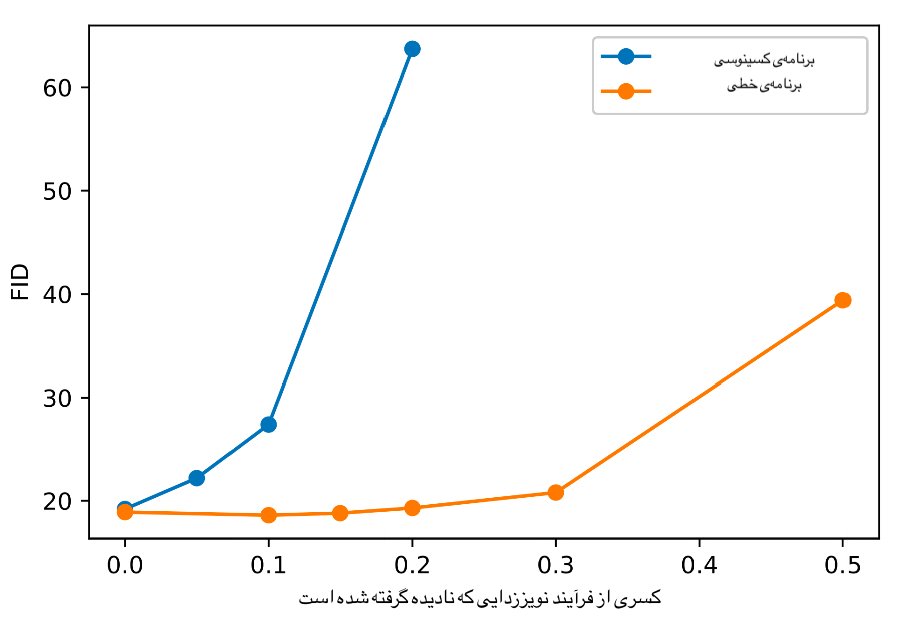
\includegraphics[width=11cm,height=8cm]{ddpm4.png}
		
		\caption{تفاوت برنامه‌ی نویز خطی و کسینوسی در حذف بخشی از فرآیند نویززدایی}
		\medskip
		\label{ddpm4}
		\small
		در مدلی که با نویز خطی پخش شده است، نادیده گرفتن ۲۰ درصد از فرآیند معکوس تاثیر مخربی بر کیفیت نمونه ها نمی‌گذارد در حالیکه در مدل کسینوسی حذف هر کسری از فرآیند معکوس کیفیت را بدتر می‌کند\cite{nichol2021improved}.
		
	\end{center}
\end{figure}

برای حل این مشکل می‌توانیم از انواع دیگری از برنامه‌های نویز مانند برنامه‌ی نویز کسینوسی استفاده کنیم.
همان طور که در شکل \ref{ddpm3} می‌بینید، این برنامه‌ی نویز با سرعت آهسته‌تری از برنامه‌ی نویز خطی به تصویر نویز اضافه می‌کند. همچنین همانطور که در شکل \ref{ddpm4} قابل مشاهده است حذف بخشی از فرآیند رو به عقب در این برنامه‌ی نویز باعث افت کیفیت تصویر می‌شود.
